\section{Physikalische Grundlagen}

\subsection{Helium-Neon-Laser}

\begin{figure}[H]
\begin{center}
  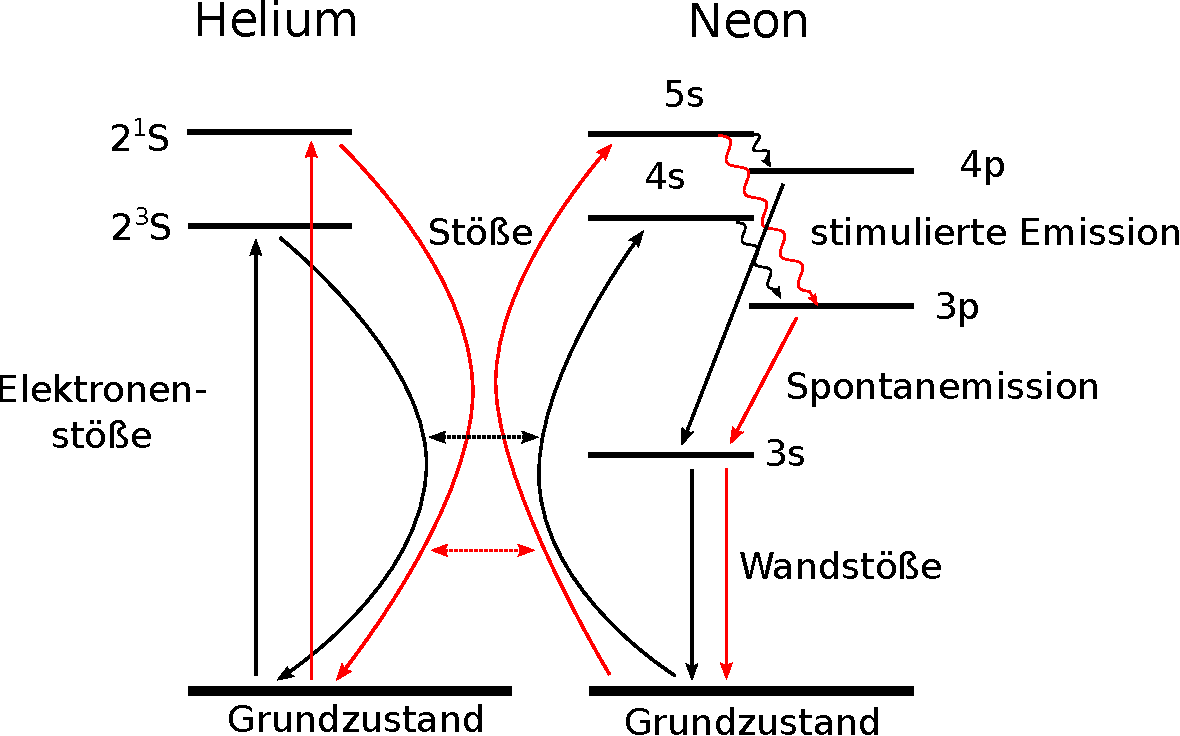
\includegraphics[width=0.8\textwidth]{../img/HeNe.pdf}
  \caption{Termschemata von Helium und Neon: Energieübergänge im Laser.
  In rot der Zyklus, der im Versuch verstärkt wird.}
  \label{img:HeNe}
\end{center}
\end{figure}

%TODO cite Demtr

Ein Laser besteht aus drei Komponenten: Einer \emph{Pumpe},
die in einem \emph{aktiven Medium} Besetzungsinversion verursacht und \emph{Spiegeln},
die emittierte Strahlung zurück in das Medium reflektierten.
Die reflektierte Strahlung stimuliert im Medium Emission und verstärkt sich dadurch selbst.\\
Der im Versuch verwendete Laser ist ein Helium-Neon-Gaslaser.
Der eigentliche Laserübergang findet beim Neon statt, das Helium dient nur zur Übertragung der Energie
auf das Neon:
Eine an der Röhre angelegte Spannung führt zu Gasentladung und Anregung der Heliumatome
in den metastabilen 2S-Zustand
(siehe \autoref{img:HeNe}).
Durch Stöße wird diese Energie auf Neonatome übertragen und diese in höhere s-Zustände angeregt.\\
Auf dem Rückweg in den Grundzustand können mehrere Übergänge als Laserübergänge verstärkt werden.
Am Versuchsaufbau wird durch geeignete Wahl der Spiegel
der Übergang 5s-3p verwendet, der eine Wellenlänge von 632.82\,nm besitzt.
Vom 3p-Zustand aus fallen die Neonatome schnell wieder spontan auf das 3s-Niveau und von dort aus
durch Wandstöße zurück in den Grundzustand.



\subsection{Der Mitführungskoeffizient als Konsequenz der speziellen Relativitätstheorie}

Taylor
Doppler-Disp


\subsection{Bestimmung des Mitführungskoeffizienten mit dem Ringlaser}


Formel für $\alpha$ mit Verweis auf Stex